

\chapter{Methods}
\label{chapter:solutions}


This Chapter has the following structure. Section \ref{section:acquisition}
describes methods of BTF acquisition and reviews some of the publicly available BTF datasets.
 Section \ref{section:compression_and_decompression} argues about the choice of compression methods, while
  Section \ref{section:pca} defines our chosen compression method.
 Section \ref{section:interpolation} defines a solution for viewing and illumination angle interpolation.
The last Section \ref{section:streaming}
concludes the Chapter with proposing our web-socket streaming model. 

\section{BTF Acquisition}
\label{section:acquisition}

BTF acquisition is not a trivial task, since to get an accurate and reliable BTF data, it is required to have an efficient BTF measurement system. 
A pioneer in this task were Dana et. al. \cite{curetDataBase}, who measured 61 materials with fixed light and moving around camera that photographed a flat surface of a material.
Such procedure results in a set of images, i.e. BTF, which can be regarded as a 6D reflectance field function \cite{sattler-2003-efficient} 

{\centering $L=L(x,y,\theta _{i},\phi _{i},\theta _{o},\phi _{o})$ \\}


where $(x,y)$ is a surface point of a flat sampled material, $(\theta _{i},\phi _{i})$ incoming light direction (light direction) and $(\theta _{o},\phi _{o})$ outgoing light direction (camera direction).

For each measured surface Dana et. al. used 205 different combinations of viewing and illumination directions. The resulted BTF can be gigabytes in size. To achive reasonable real-time performance compression of BTF
is an inevitable step. Also, Dana's et. al. BTF database is not spatially registered, i.e. images were not mutually registered for different view angles. That means one should further process the database in order to render BTF.

Based on Dana et. al. BTF measurement system, Sattler from Bonn University made his own measuring system \cite{sattler-2003-efficient}. The main difference in that system is that a camera moves on a semi-circle rail around a material.
Also, such setup provides spatially registered data, with reasonable angular and spatial resolutions. Datasets of Bonn University \cite{btfBonn} are publicly available and were used in this thesis.



\begin{figure}[h]
 \centering
 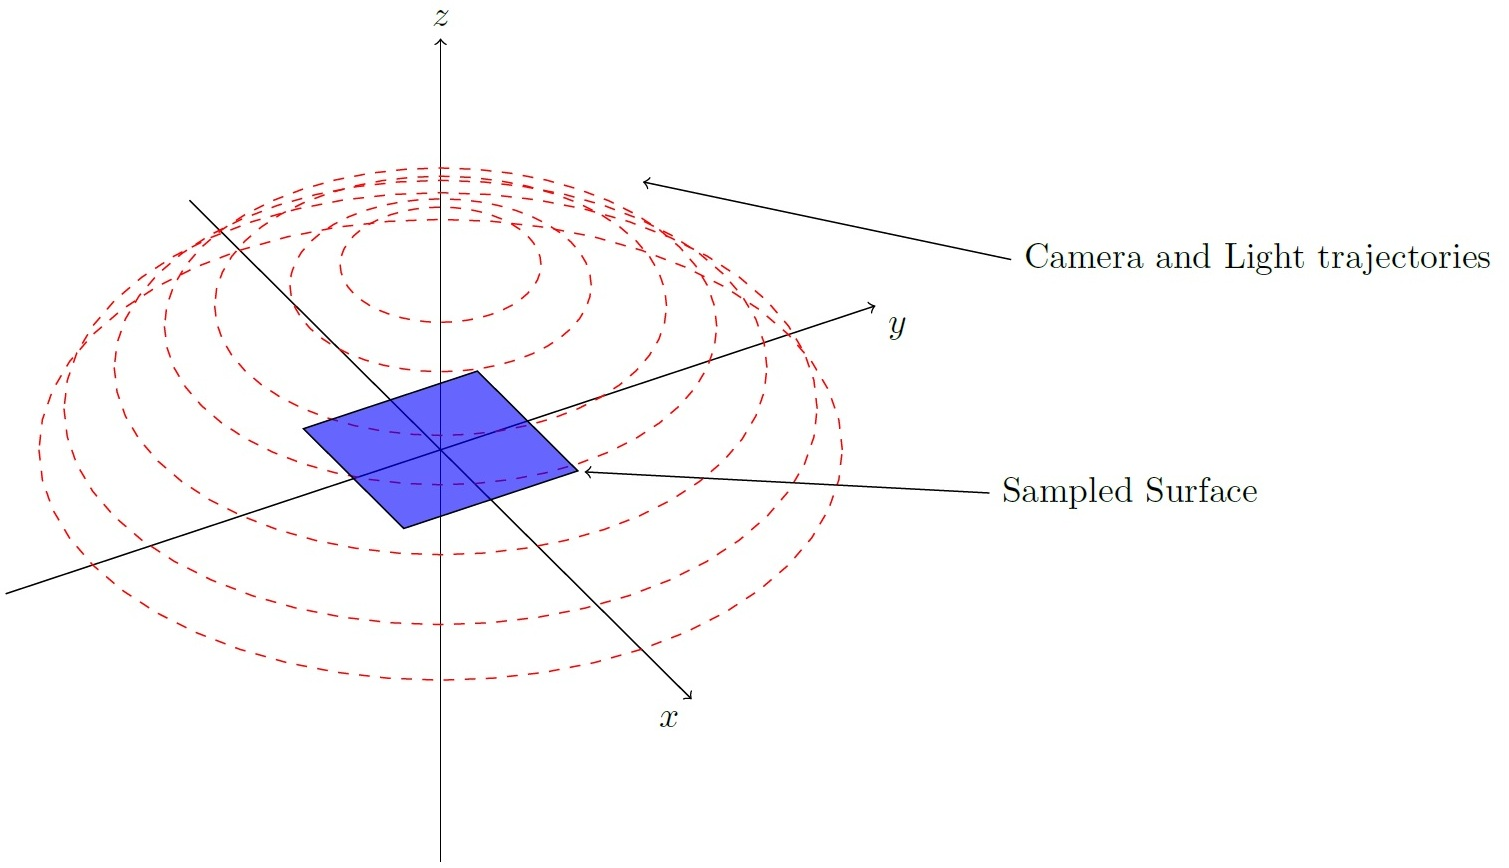
\includegraphics[width=1.0\textwidth]{figures/acquisition}
 \caption[Example of BTF measurement] {
 	{\bf Example of BTF measurement.}

	Camera and light positions share the same trajectories.
	Red dashed circles are the sample positions on the hemisphere. }
 \label{fig:acquisition_example}
\end{figure}


 Consider Figure \ref{fig:acquisition_example}, which illustrates one of the possible ways of sampling the material.
The measured surface is being fixed all the time on the sampler holder. Then, for each light position, a camera photographs the flat material while moving from point to point of the hemisphere.
Bonn database has the same trajectory for camera and light positions, i.e. 81 positions on the hemisphere, which results in 6561 total number of acquired images.



\begin{figure}[h]
 \centering
 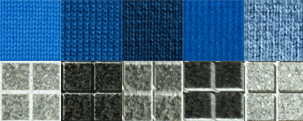
\includegraphics[width=1.0\textwidth]{figures/exampleBTF}
 \caption[Example of BTF measurement] {
 	{\bf BTF example of Bonn Database \cite{btfBonn}.}

	Example how BTF catches rich appearance of the material due to dependencies on light and camera views. 
	Upper row is a knitted wool, lower is a graved granite stone.}
 \label{fig:exampleBTF}
\end{figure}



\section{Compression and Decompression}
\label{section:compression_and_decompression}

As we already know BTF is a high dimensional data, which makes it enormous in size.
Datasets of Bonn are 8-bit PNG images with $256\times256$ resolution.
 Then, after an uncompressed PNG data loads to GPU it occupies approx. 1,2 GB of space. And that's not even large a spatial resolution in this case!
 Therefore, it is impractical to render BTF as a raw data even on the most modern GPUs.
 
 The most common technique to compress BTF is Principal component analysis (PCA), which is widely used in image compression \cite[Ch.\ 15]{haindl,gpu_gems}.
 PCA were used in several works of Bonn University \cite{sattler-2003-efficient,mueller-2003-compression,mueller-2004-environmental}.
 Also, at some point PCA were employed as a basis for Decorrelated Full Matrix Factorization compression method \cite{webglbtfstreaming}.
 
 The reason that PCA is the broadly used is because a user can straightforwardly change parameters of the model and control a trade between compression ratio and a reconstructed image quality.
 Unlikely, other methods based on probabilistic MRF models \cite{haindl}, even though probabilistic  methods provide thousand times better compression rate than linear factorization methods.
 Also, one more advantage of PCA is that is more suitable for low-end GPUs, because for example MRF methods can be very heavy for GPU.
 
 
\subsection{PCA}
\label{section:pca}

By a common definition Principal component analysis (PCA) is a mathematical tool that reduces the dimensions of possibly correlated variables. New reduced dimensions are called \emph{principal components}.
Principal components hold the most important variations of the data, e.g. first ones hold the biggest amount of texture details. Using principal components it is possible to reconstruct the whole data. 
Due to neglecting small variations of the variables at first place, the reconstructed data will differ from original one, but the most important variations of the data will be preserved. 
That's why PCA is good for image compression, because a human eye is not that sensitive to small variations, i.e. reconstructed image might look almost the same as original for an observer.
The good part about losing small variations, is that we can reduce some noise that was present in the original images \cite{pca_noise}.
\subsection{Data representation}
\label{section:first_step}

First step in our analysis is to chose a suitable data representation. Basically, there are two common arrangements, i.e. as a set of images or BRDFs (Bidirectional reflectance distribution function). 
Both representations can be mathematically interpreted as  \cite{mueller-2003-compression}


{\centering $\,\,BTF_{BRDF} \;\, = \left \{ {P_{(x)}} \right \}_{(x)\in I\subset \mathbb{N}^{2}}$ \\}
{\centering $BTF_{Image}=\left \{ I_{(v,l)} \right \}_{(v,l)\in M}$\\}

where $M$ denotes a set of images $I_{(v,l)}$ measured for different view and light directions $(v,l)$ accordingly.
$BTF_{BRDF}$ denotes a set of $P_{(x)}$ images, where each of them depends on a single spatial position $x$ for all possible views, i.e. $ \forall (v,l):x \in I_{(v,l)}$.
Note that such BRDFs are not fulfilling physical demanded property such as reciprocity, because they already contain a factor between an incident light direction and a normal, i.e. $n*l$.
In our case with Bonn datasets the sizes of variable vectors which we want to compress are $\left | I \right | = 3\times256\times256$ and $\left | M \right | = 3\times81\times81$, where $3$ stands for RGB channels.


M{\"u}ller et. al. \cite{mueller-2003-compression, haindl} claim that BRDF representation works slightly better in comparison to image-wise. 
The advantage of BRDF is that a compression ratio can be 10 times better and reconstruction error is slightly smaller than the image-wise representation.
Also, Borshukov et. al. \cite[Ch.\ 15]{gpu_gems} chose BRDF representation, claiming that it provides better compression ratio.
The reason why BRDF provides better compression ratio is because it provides better pixel-to-pixel comparison than image-wise. 
Each variable vector of BRDF arrangement depends only on a surface complexity \cite{mueller-2003-compression}, i.e. 
on a variation of reflection properties at a spatial point of the surface.
On the contrary, image-wise variable depends on the whole measured image plane, thus it is logical that it may provide lower compression rate due to stronger variations.
After all, we have chosen BRDF data representation based on such reasons, with which we have achieved $1:100$ compression ratio. 

\subsection{Algorithm}
\label{section:algorithm_step}
The algorithm of PCA for BTF compression and decompression is mainly borrowed from  Borshukov et. al \cite[Ch.\ 15]{gpu_gems}.
 Basically, this is a common algorithm of PCA that deploys computing a singular value decomposition (SVD).

In the \emph{first} step of algorithm we built BRDF representation of the BTF data.
Let matrix $A$ denote the stored BTF data.
We consider each image $I$ as three column vectors $a_{i}$ (red, green, and blue channels), where $i=0..3*N$. $N$ is the number of images.
The size of $a_{i}$ is $W\times H$, where $W$ and $H$ are dimensions of the image.
So, matrix $A$ has the following dimensions $(W*H)\times(3*N)$, which consist of such columns $a_{i}$.
Rows of matrix $A$ are BRDF representation of BTF, which will be dimensionally reduced.

The  \emph{second} step is called "centring" of the data. We compute the average value of each row of matrix $A$

{\centering $m_i=\frac{1}{3N}\sum_{i=1}^{3N}A_{i,j}$ \\}

Then, we subtract mean vector from each column of matrix $A$

{\centering $B_{i,j}=A_{i,j}-m_i.$ \\}

At the \emph{last} step, we compute singular value decomposition (SVD) of matrix $B$. The result of which will be such decomposition

{\centering $B=U\Sigma V^{T}$ \\}

where matrix $U$ holds \emph{principal components} of size $W\times H$. $\Sigma$ is a diagonal matrix and holds the "importance" value of each principal components, and
matrix $V$ stores weights that are needed for reconstructing matrix $B$.

\subsection{Compression}
\label{section:compression}




\begin{figure}[h]
 \centering
 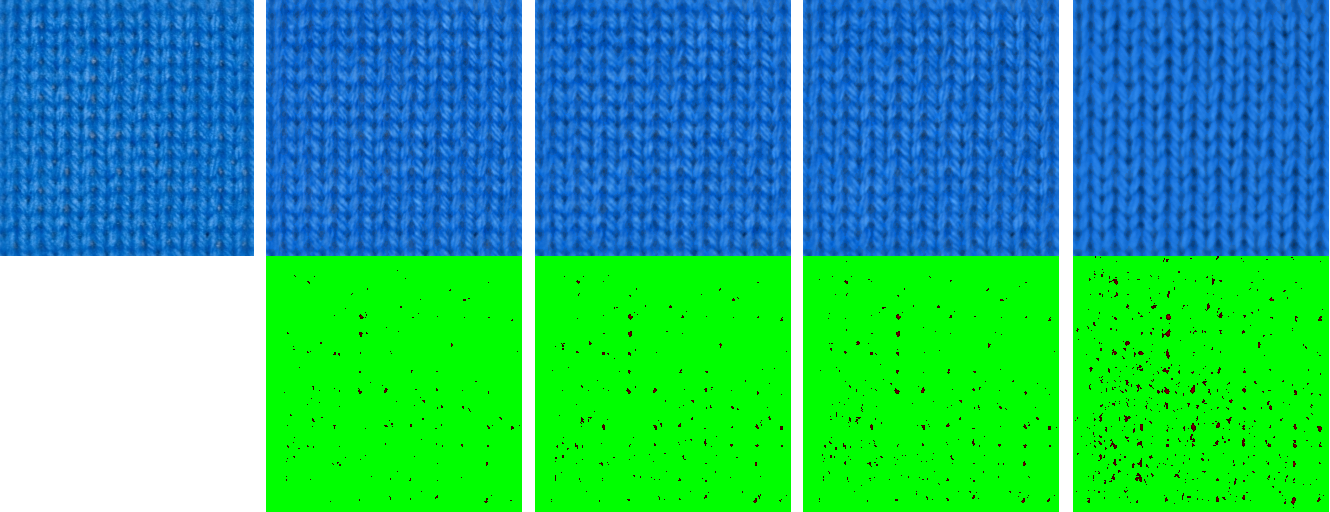
\includegraphics[width=1.0\textwidth]{figures/differ0}
 \caption[Example of compression ] {
 	{\bf Example of compression \textnumero 1.}

	\textbf{First row} from the left to the right: original image, \textbf{32} components (RMSE:7.7\%), \textbf{16} components (RMSE:8.2\%), \textbf{8} components (RMSE:8.5\%), \textbf{4} components (RMSE:10\%). 
	
	\textbf{Second row}: the difference between original and decompressed, \emph{red} color denotes how big the error, \emph{green} denotes that error is absent or very small.}
 \label{fig:compression_example_1}
\end{figure}



In order to achieve good compression ratio and at the same time preserve a decompressed quality we need to chose suitable parameters for PCA.
We perform PCA on subsets of 81 camera views. For each camera view there are 81 images sampled for different light directions.
We take $3$ neighbour views at once and perfrom PCA on them. With such size of subset we can achieve good trade between quality and compression ratio.
 For subsets of size $1$ RMSE (Root mean square error) improves to 5\%-7\% on average.
If we want to achieve even bigger compression ratio we can make the size of the subset even bigger, but of course the quality of decompressed texture will be worse compared to smaller subset sizes.
Also, performing PCA on the bigger subsets is inefficient, e.g. the time required to perform PCA on all $81$ views at once can take hours and memory requirements to compute SVD are demanding.


Consider examples  shown in Figure \ref{fig:compression_example_1}. We can see that for $4$ components all images are getting blurred.
In our case, $8$ components is a reasonable choice, as even for $32$ components the quality improvement is not that visible. Besides, smaller number of components will make decompression performance better.


The second example in Figure \ref{fig:compression_example_2} has worse reconstructed quality than in Figure \ref{fig:compression_example_1} due to small specularities on the surface, which are not preserved in principal components.
This example demonstrates the limitation of PCA, i.e. such small details may not be reconstructed.
But, an overall structure and a tone of the texture is preserved.
Also, compression ration 1:100 is achieved with such parameters, i.e. from 1,2 GB we now store around 20 MB in GPU.




\begin{figure}[h]
 \centering
 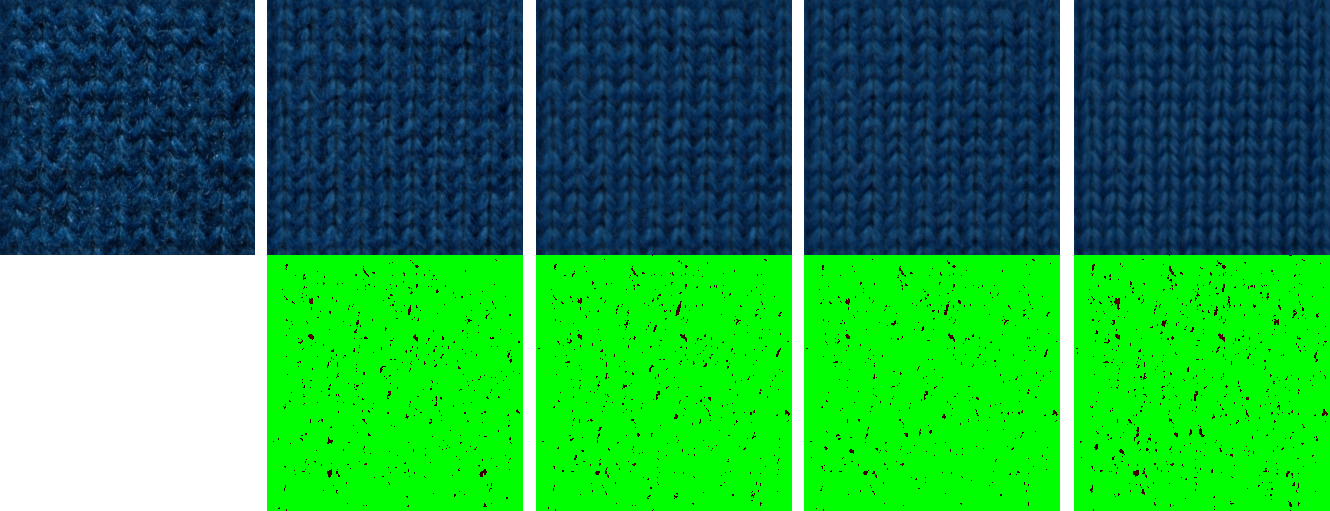
\includegraphics[width=1.0\textwidth]{figures/differ}
 \caption[Example of compression ] {
 	{\bf Example of compression \textnumero 2.}

	\textbf{First row} from the left to the right: original image, \textbf{32} components (RMSE:8.3\%), \textbf{16} components (RMSE:8.4\%), \textbf{8} components (RMSE:8.2\%), \textbf{4} components (RMSE:9.2\%). 
	\textbf{Second row}: the difference between original and decompressed, \emph{red} color denotes how big the error, \emph{green} denotes that error is absent or very small.}
 \label{fig:compression_example_2}
\end{figure}

\subsection{Decompression}
\label{section:Decompression}
The decompression step is simply matrix operations, which require to combine 3 matrices $U$, $\Sigma$, $V$ and mean vector $m$.
To make it a bit easier to decompress on GPU we construct new matrices as Borshukov et. al.

{\centering $L=\begin{bmatrix}
 m\mid U \Sigma
\end{bmatrix}$ \\}

{\centering $
R=\begin{bmatrix}
 1 ... 1   \\ 
  \, \, \, V^{T}
\end{bmatrix}.$ \\}
  Matrix $A$ takes such form of decompression $A=LR$. In detail, if want to decompress texture with index $i$ for first $C$ components, we do it separately for each color channel


{\centering $red(x,y)=\sum_{k=1}^{C}L_{xy,k}R_{k,3i+0}$ \\}
{\centering $green(x,y)=\sum_{k=1}^{C}L_{xy,k}R_{k,3i+1}$ \\}
{\centering $blue(x,y)=\sum_{k=1}^{C}L_{xy,k}R_{k,3i+2}$ \\}


\section{Viewing and Illumination Angle Interpolation}
\label{section:interpolation}

BTF datasets are measured for discrete number of angles, thus we would need to perform interpolation for unknown not measured angels.
We will employ barycentric coordinates interpolation. 
However, it is very computational heavy, so the following approximation algorithm proposed by Hatka and Haindl \cite{btfblender} will be used.

Assume that we have found triangle $P_{1}P_{2}P_{3}$ which bounds our point P, which we want to interpolate. Figure \ref{fig:acquisition_example} demonstrates hemisphere on which triangle $P_{1}P_{2}P_{3}$ lies.
$Y_{P}$ denotes desired pixel color. 
So, generally speaking linearly interpolation of that pixel will be $Y_{P}=w_{1}Y_{P1} + w_{2}Y_{P2} + w_{1}Y_{P2}$, 
where $Y_{P1},Y_{P2},Y_{P3}$ correspond to measured pixel color of positions $P_{1},P_{2},P_{3}$ accordingly. Weights $w_{1},w_{2},w_{3}$ are normalized and sum up to $1$.

Weights defined as volumes $V_{1},V_{2},V_{3}$ which correspond to $PP_{2}P_{3}O$, $PP_{3}P_{1}O$, $PP_{1}P_{2}O$ tetrahedrons, where $O=(0,0,0)$.
All volumes are normalized, which means $V_{i}=\frac{V_{i}}{\sum_{i=1}^{3}V_{i}}$. Volumes calculated as determinates of $4\times 4$ vectors

{\centering $V_{1}=\frac{1}{6}\left | det(PP_{2}P_{3}O) \right |$ \\}
{\centering $V_{2}=\frac{1}{6}\left | det(PP_{3}P_{1}O) \right |$ \\}
{\centering $V_{3}=\frac{1}{6}\left | det(PP_{1}P_{2}O) \right |$ \\}

\section{Streaming}
\label{section:streaming}


The size of compressed BTF data using PCA is around 10-20 Mb on a hard drive. 
Even though, compressed BTF data size is sufficient for plausible rendering, it is still big enough for transferring it over the internet for web rendering.
The full transfer of BTF may take some minutes, especially with slow internet connection. To make this process faster and rendering a bit more interactive, we will use progressive streaming of BTF data.
Deploying streaming a user will be able to see a preview of original BTF just in a few seconds. 
Principal components will be streamed one by one using WebSockets \cite{websockets} and rendering will be refreshed whenever a new component arrives.
The quality will be progressively improved during streaming, see Figure \ref{fig:streamPreview} for an example. Also, it is possible to show an overall progress for the user, which makes the process of streaming even more interactive.


We use WebSockets for streaming the data, as it is most efficient and elegant way of communicating between a server and a client nowadays.
The following advantages of WebSocket technology \cite[Ch.\ 1]{websockets} are:

\begin{itemize}
  \item \textbf{Delivers high \emph{Performace}}  for real-time server-client connections. 
  Usually, web developers used well known methods such as polling, long polling, and HTTP streaming. However, WebSocket saves bandwidth, CPU power, and latency compared to those methods.
  For example, polling method makes requests to the server and has to wait for the response.
  With WebSockets the client does not need to wait for the response, because WebSockets reuse the same connection from client to the server and wise-verse.
  This single connection reduces the latency.

  \item \textbf{\emph{Saves time}} to develop web-applications. \emph{Simplicity} of is one of the main advantage over older methods for server-client communication.
  
\end{itemize}

\begin{figure}[h]
 \centering
 \includegraphics[width=1.0\textwidth]{figures/streampreview}
 \caption[Example of Progressive Streaming ] {
 	{\bf Example of Progressive Streaming}

	\textbf{From left to right}: \emph{1}, \emph{2}, \emph{4}, \emph{6}, \emph{7}  components rendered at the same time.
	
	\textbf{Note}: \emph{8th} component is a mean value $m_{i}$, which sends at the first place.
	}
 \label{fig:streamPreview}
\end{figure}


As it was described in Section \ref{section:algorithm_step} matrices $U$, $\Sigma$, $V$ and $m_{i}$ store all the needed data to reconstruct BTF.
Matrices $\Sigma$ and $V$ are quite small in size, they are sent at first place. On the contrary, matrix $U$ stores principal components of size $W \times H$ which makes matrix $U$ the biggest in size of all.
Matrix $U$ also stores mean values $m_{i}$ as first component.
After a Socket connection was established, the client side requests one component at a time. 
Each newly arrived component saved in matrix $U$ and the client side refreshes the shader to render BTF.



Consider Figure \ref{fig:streamPreview} that shows how the streaming works on practice.
We can see that even with first components the resulted texture looks quite decent.
With further components the overall quality of texture improves, e.g. specularities are increasing, small micro-structures become more visible and emphasized.
To make the streaming process a bit entertaining, the client also can see the progress-bar of the streaming progress.









